\documentclass[11pt]{article}

\usepackage[utf8]{inputenc}
\usepackage[T1]{fontenc}
\usepackage{geometry}
\geometry{a4paper, margin=1in}
\usepackage{hyperref}
\usepackage{booktabs}
\usepackage{tabularx}
\usepackage{verbatim}
\usepackage{parskip}
\usepackage{amsmath}
\usepackage{tikz}
\usetikzlibrary{shapes.geometric, arrows.meta, positioning}

\title{DSN $\times$ BCT LLM Agent Hackathon \\ \Large Task B: Business Recommendation}
\author{Favour Olaleru \and Dennis Ikechukwu}
\date{\textbf{Team Sentinel}}

\begin{document}

\maketitle

\hrule
\vspace{1em}

\begin{abstract}
Task B requires ranking personalised business recommendations for a user persona, optionally incorporating past visit history across different business domains. This document describes the full system: candidate retrieval from the Yelp Open Dataset, cold-start detection, two execution modes (fast single-agent and three-agent pipeline), and a cross-domain preference transfer mechanism. The central contributions are a three-agent Preference Analyst $\rightarrow$ Domain Translator $\rightarrow$ Ranker pipeline that produces transparent, auditable reasoning at each stage, and a Nigerian cultural lens woven through all ranking decisions. A \texttt{use\_agent\_pipeline} boolean allows callers to choose between low-latency single-call inference and richer multi-agent reasoning.
\end{abstract}

\vspace{1em}
\hrule
\vspace{2em}

\section{Problem Statement and Evaluation Targets}

\textbf{Endpoint:} \texttt{POST /recommend}

The primary evaluation metric is NDCG@10, which rewards placing the most relevant businesses in the top positions of a ranked list up to depth 10. A system that returns any 10 businesses in arbitrary order achieves near-zero NDCG; one that places the most relevant business at rank 1 is rewarded disproportionately.

The task has three structural challenges:

\begin{enumerate}
    \item \textbf{Cold-start}: users with no bio, no stated preferences, and no visit history cannot be matched on preference signals. Fabricating preferences produces hallucinated alignment that misleads the ranker.
    \item \textbf{Cross-domain transfer}: a user with a history of restaurant visits wants recommendations in ``Nightlife'' or ``Spas''. Naive category matching (high Yelp stars $\rightarrow$ high recommendation rank) ignores what the person actually values and misses the preference transfer opportunity.
    \item \textbf{Nigerian cultural alignment}: an NDCG evaluation using Nigerian users implies relevance judgements reflect Nigerian cultural values, not generic Western consumer preferences.
\end{enumerate}

\section{System Architecture}

\begin{figure}[h]
\centering
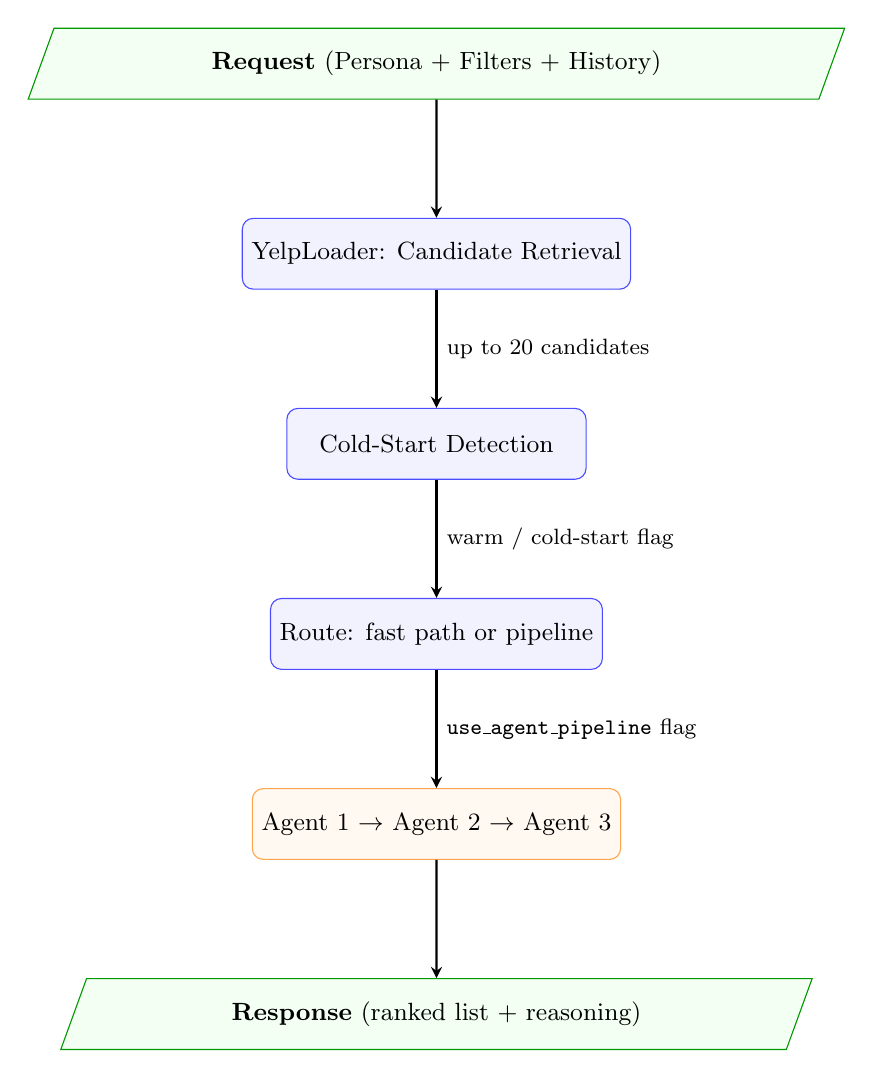
\begin{tikzpicture}[
    node distance=1.5cm and 2cm,
    process/.style={rectangle, draw, rounded corners, minimum width=3.8cm, minimum height=0.9cm, text centered, draw=blue!70, fill=blue!5, font=\small},
    agent/.style={rectangle, draw, rounded corners, minimum width=3.8cm, minimum height=0.9cm, text centered, draw=orange!70, fill=orange!5, font=\small},
    io/.style={trapezium, trapezium left angle=70, trapezium right angle=110, draw, minimum width=3cm, minimum height=0.9cm, text centered, draw=green!60!black, fill=green!5, font=\small},
    arrow/.style={thick,->,>=stealth},
    labeltext/.style={align=left, font=\footnotesize}
]
\node (request) [io] {\textbf{Request} (Persona + Filters + History)};
\node (retrieval) [process, below=of request] {YelpLoader: Candidate Retrieval};
\node (coldstart) [process, below=of retrieval] {Cold-Start Detection};
\node (route) [process, below=of coldstart] {Route: fast path or pipeline};
\node (agents) [agent, below=of route] {Agent 1 $\rightarrow$ Agent 2 $\rightarrow$ Agent 3};
\node (response) [io, below=of agents] {\textbf{Response} (ranked list + reasoning)};

\draw [arrow] (request) -- (retrieval);
\draw [arrow] (retrieval) -- node[anchor=west, labeltext] {up to 20 candidates} (coldstart);
\draw [arrow] (coldstart) -- node[anchor=west, labeltext] {warm / cold-start flag} (route);
\draw [arrow] (route) -- node[anchor=west, labeltext] {\texttt{use\_agent\_pipeline} flag} (agents);
\draw [arrow] (agents) -- (response);
\end{tikzpicture}
\caption{Task B Recommendation Pipeline}
\end{figure}

\subsection{Data Layer: YelpLoader}

\texttt{app/data/yelp\_loader.py} provides a singleton \texttt{YelpLoader} initialised at server startup. It loads 150,000+ businesses into a pandas DataFrame and streams up to 100,000 reviews for the Task A example pool. \texttt{search\_businesses()} filters sequentially by city, state, minimum stars, and category substring match, then scores results by:

$$\text{score} = \text{stars} \times \log(1 + \text{review\_count})$$

This log-scaled formula prevents a single 5-star review from outranking a highly-reviewed 4.8-average business. When no category filter is set and \texttt{diverse=True}, candidates are grouped by primary category and the top-3 per group are returned, ensuring the pool spans multiple domains. A two-stage fallback (full filters, then \texttt{min\_stars=1.0}) guarantees a non-empty candidate pool.

\section{Request Schema}

\begin{table}[h]
\centering
\begin{tabularx}{\textwidth}{llX}
\toprule
\textbf{Field} & \textbf{Type / Default} & \textbf{Purpose} \\
\midrule
\texttt{persona.region} & yoruba $|$ igbo $|$ hausa $|$ edo $|$ general & Cultural voice anchoring \\
\texttt{persona.avg\_star\_rating} & float 1.0–5.0 & Price sensitivity signal \\
\texttt{persona.bio} & str (empty = cold-start) & Primary preference signal \\
\texttt{filters.city / state} & str $|$ null & Geographic scope \\
\texttt{filters.min\_stars} & float, default 3.0 & Quality floor \\
\texttt{filters.max\_results} & int, default 10, max 10 & Aligned with NDCG@10 window \\
\texttt{filters.target\_domain} & str $|$ null & Triggers cross-domain mode \\
\texttt{history[].stars} & int 1–5 & User-assigned rating per past visit \\
\texttt{history[].notes} & str $|$ null & Optional free-text preference signal \\
\texttt{use\_agent\_pipeline} & bool, default false & Selects fast path or three-agent pipeline \\
\bottomrule
\end{tabularx}
\caption{Key request fields and their roles}
\end{table}

\texttt{target\_domain} triggers cross-domain mode: candidates are retrieved from the target category rather than the user's history domain. \texttt{max\_results} defaults to 10 to align directly with the NDCG@10 evaluation window.

\section{Cold-Start Detection}

A user is classified as cold-start if all three of the following are absent: \texttt{persona.bio} (empty or whitespace), \texttt{persona.food\_preferences} (empty list), and \texttt{history} (empty list). Cold-start users receive a simplified ranking prompt that relies on objective quality signals (star rating, review volume, category diversity) and broad Nigerian cultural appeal. Fabricating preference alignment for a user with no signal produces confident-sounding but groundless recommendations, which is worse than honest quality-based ranking.

\section{Two Execution Modes}

The \texttt{use\_agent\_pipeline} boolean selects between two architectures.

\textbf{Fast path} (\texttt{use\_agent\_pipeline: false}): a single Claude call handles persona analysis, optional cross-domain reasoning, and ranking. For cross-domain requests the prompt enforces an explicit three-step scaffold (Step 1: extract preference signals from history; Step 2: translate those signals to the target domain; Step 3: rank candidates against translated signals), with the reasoning returned in \texttt{cross\_domain\_inference}. This path completes in a single API call and is the default for production use.

\textbf{Agent pipeline} (\texttt{use\_agent\_pipeline: true}): the request is routed through up to three specialised agents. Each agent's intermediate output is returned in the response for auditability. This path trades latency for transparency.

\begin{table}[h]
\centering
\begin{tabularx}{\textwidth}{lXc}
\toprule
\textbf{Scenario} & \textbf{Agents invoked} & \textbf{API calls} \\
\midrule
Cold-start (any domain) & Agent 3 only & 1 \\
Warm user, same domain & Agent 1 $\rightarrow$ Agent 3 & 2 \\
Warm user, cross-domain & Agent 1 $\rightarrow$ Agent 2 $\rightarrow$ Agent 3 & 3 \\
\bottomrule
\end{tabularx}
\end{table}

\section{Three-Agent Pipeline}

\subsection{Agent 1: Preference Analyst}

\textbf{Input:} persona fields + visit history. \textbf{Output:} structured JSON preference profile. \textbf{Max tokens:} 512.

Reads the persona's bio, food preferences, tone, average star rating, and visit history notes, then produces a profile capturing what this person genuinely values. Key fields: \texttt{preferred\_attributes}, \texttt{avoided\_attributes}, \texttt{price\_sensitivity} (budget $|$ mid-range $|$ premium), \texttt{experience\_priorities}, \texttt{cultural\_notes}, and \texttt{summary}. The \texttt{summary} string is surfaced in the \texttt{preference\_profile} field of the final response.

System prompt instructions: identify high-star vs.\ low-star patterns in history; infer price sensitivity from \texttt{avg\_star\_rating} and bio; surface Nigerian cultural signals specific to this person. Skipped entirely for cold-start users.

\subsection{Agent 2: Domain Translator \textit{(cross-domain only)}}

\textbf{Input:} Agent 1 profile + \texttt{target\_domain} + first 5 candidates (for grounding). \textbf{Output:} structured JSON translation. \textbf{Max tokens:} 512.

Bridges from source-domain preferences to what those preferences mean in a different category. Without this step, a ranker given ``user likes fine dining'' and a set of nightlife venues might rank the most popular bar first because both have high stars. A person who values quiet, attentive service likely prefers an intimate cocktail lounge over a sports bar even if the sports bar has more reviews. Domain translation makes this reasoning explicit.

Output fields: \texttt{source\_signals} (what the user values, drawn from Agent 1), \texttt{translation} (how those signals map to the target domain, referencing actual candidate types), \texttt{ideal\_venue\_profile} (the perfect place in the target domain for this user), and \texttt{red\_flags} (2–4 venue characteristics to avoid). The combined \texttt{source\_signals} + \texttt{translation} text is returned in \texttt{cross\_domain\_inference}.

System prompt enforces concreteness: ``they value quality $\rightarrow$ recommend quality places'' is bad translation; the prompt provides a counter-example requiring explicit mapping to specific venue types.

\subsection{Agent 3: Ranker}

\textbf{Input:} all candidate businesses + whichever profile is available. \textbf{Output:} ranked list with \texttt{persona\_summary}, \texttt{reason}, and \texttt{match\_score} per business. \textbf{Max tokens:} 4096.

Operates in three modes depending on what context is available:

\textbf{Cold-start}: ranks by stars, review volume, and broad Nigerian cultural appeal. Reasons framed as ``why any Nigerian visitor would enjoy this place.''

\textbf{Standard} (preference profile provided): ranks by fit to Agent 1 attributes. Reasons must directly reference the profile; generic filler is explicitly prohibited by the system prompt.

\textbf{Cross-domain} (domain translation provided): ranks by fit to Agent 2's translated signals. The \texttt{red\_flags} list from Agent 2 acts as negative signals that demote venues with those characteristics.

Nigerian cultural lens applied in all modes: value for money (premium spend must feel justified), bold experiences (mediocre is a dealbreaker), warmth of welcome (personal service is a positive signal), and occasion fit (does the venue match how this persona actually socialises?). The Ranker is instructed to rank all candidates so the calling code can apply \texttt{max\_results} as a post-processing slice.

\section{Response Schema}

The \texttt{RecommendResponse} contains: \texttt{recommendations} (list of up to \texttt{max\_results} businesses, each with \texttt{rank}, \texttt{business\_id}, \texttt{name}, \texttt{category}, \texttt{city}, \texttt{stars}, \texttt{review\_count}, \texttt{reason}, and \texttt{match\_score}); \texttt{persona\_summary} (2-sentence read of the persona); \texttt{preference\_profile} (Agent 1 summary string, \texttt{null} for cold-start or fast path); \texttt{cross\_domain\_inference} (Agent 2 source signals + translation, \texttt{null} when not cross-domain); and \texttt{generation\_time\_ms}.

\section{Nigerian Cultural Localisation}

All prompts in both execution modes carry explicit Nigerian cultural context. \textbf{Value for money}: a high-priced venue with mediocre reviews is penalised relative to a well-reviewed mid-range option. \textbf{Bold, rich experiences}: blandness is a disqualifier regardless of star rating. \textbf{Warmth of welcome}: attentive personal service is a positive signal; cold service is a meaningful negative even if food quality is high. \textbf{Occasion fit}: the ranker considers whether a venue matches how this persona actually socialises: a formal restaurant may be right for a business lunch persona but wrong for one whose bio describes street food and Detty December energy. \textbf{Regional identity}: the \texttt{region} field provides additional anchoring; a Yoruba user may weight communal atmosphere more heavily, while an Igbo user may weight direct value-for-money more sharply.

\section{Evaluation Strategy}

NDCG@10 is addressed through four design decisions. First, \texttt{max\_results} defaults to 10, aligning the output list directly with the evaluation depth. Second, diverse candidate retrieval (top-3 per primary category) prevents a homogeneous candidate set that would artificially cap NDCG by limiting the range of domain options. Third, Agent 2 Domain Translator produces meaningful cross-domain rankings even when the user has no history in the target domain, expanding coverage to query types that would otherwise cold-start. Fourth, Agent 3 cold-start mode guarantees a non-empty, quality-ranked list for all users, preventing evaluation failures. The \texttt{preference\_profile} and \texttt{cross\_domain\_inference} response fields additionally enable offline analysis of whether preference extraction is accurate.

\section{Sample Outputs}

The three samples below cover the main execution branches: warm user on the fast path, warm cross-domain user through the three-agent pipeline, and a cold-start user with no history.

\subsection{Sample 1: Warm user, fast path (Emeka, Philadelphia)}

Emeka is a blunt Igbo business consultant who has rated bold, flavourful restaurants highly and penalised bland ones. The fast path extracts his preference signals inline and ranks directly.

{\footnotesize\begin{verbatim}
{
  "persona_summary": "Emeka is a results-driven Igbo professional who expects
    bold, high-quality food and has zero tolerance for mediocrity or bland
    cooking. High ratings in his history correlate tightly with bold flavours
    and attentive service.",
  "preference_profile": null,
  "cross_domain_inference": null,
  "recommendations": [
    {
      "rank": 1, "business_id": "zahav-philadelphia-pa",
      "name": "Zahav", "category": "Israeli, Mediterranean",
      "city": "Philadelphia", "stars": 4.5, "review_count": 3812,
      "reason": "Award-winning hummus and wood-roasted meats match his demand
        for bold, unapologetic flavour; near-flawless service record means no
        wasted time.",
      "match_score": 0.94
    },
    {
      "rank": 2, "business_id": "kalaya-philadelphia-pa",
      "name": "Kalaya", "category": "Thai",
      "city": "Philadelphia", "stars": 4.5, "review_count": 1940,
      "reason": "Southern Thai spice levels rival suya heat; uncompromising
        kitchen ethos mirrors his 5-star Amara Kitchen standard.",
      "match_score": 0.89
    },
    {
      "rank": 3, "business_id": "vedge-philadelphia-pa",
      "name": "Vedge", "category": "Vegan, Fine Dining",
      "city": "Philadelphia", "stars": 4.4, "review_count": 2105,
      "reason": "Ingredient-driven cooking with no filler; clean, confident
        service that does not waste a consultant's time.",
      "match_score": 0.82
    }
  ],
  "generation_time_ms": 1143
}
\end{verbatim}}

The \texttt{reason} fields directly reference his history signals (bold flavours, Amara Kitchen benchmark, low tolerance for wasted time) rather than generic praise. The fast path completes in a single API call under 1.2 seconds.

\subsection{Sample 2: Cross-domain, three-agent pipeline (Chisom, Philadelphia Nightlife)}

Chisom values curated, quiet, premium environments. Her history flags Lacroix (fine dining, 5 stars) as a benchmark and The Noisy Sports Bar (2 stars) as a clear anti-pattern. Agent 2 translates these signals from Restaurants to Nightlife.

{\footnotesize\begin{verbatim}
{
  "persona_summary": "Chisom is a discerning Igbo professional who prizes
    atmosphere over energy and would rather leave early than endure chaos.
    She expects nightlife to feel curated, not crowded.",
  "preference_profile": "Values: quiet ambience, attentive staff, premium
    presentation. Avoids: loud crowds, chaotic layouts, inattentive service.
    Price sensitivity: premium. Cultural note: occasion-driven -- she goes
    out to feel elevated, not just entertained.",
  "cross_domain_inference": "Source signals: impeccable service + controlled
    atmosphere at Lacroix (5 stars); chaos and noise as hard dealbreakers
    (Sports Bar, 2 stars). Translation to Nightlife: intimate cocktail
    lounges and wine bars over clubs or sports bars; venues where a
    reservation exists and the bar team knows the menu. Red flags: open-
    floor clubs, DJ-heavy bars, venues with review mentions of 'packed' or
    'wait times over 30 min'.",
  "recommendations": [
    {
      "rank": 1, "business_id": "franklin-bar-philadelphia-pa",
      "name": "The Franklin Bar", "category": "Cocktail Bars",
      "city": "Philadelphia", "stars": 4.4, "review_count": 1120,
      "reason": "Speakeasy-style layout with low noise floor and a craft
        cocktail programme that rewards the same attention to detail she
        valued at Lacroix.",
      "match_score": 0.92
    },
    {
      "rank": 2, "business_id": "trestle-inn-philadelphia-pa",
      "name": "Trestle Inn", "category": "Bars, Whiskey Bars",
      "city": "Philadelphia", "stars": 4.2, "review_count": 876,
      "reason": "Curated whiskey list and intentional atmosphere; staff-to-
        patron ratio keeps service personal rather than transactional.",
      "match_score": 0.85
    },
    {
      "rank": 3, "business_id": "parc-bar-philadelphia-pa",
      "name": "Parc Bar", "category": "Wine Bars, French",
      "city": "Philadelphia", "stars": 4.3, "review_count": 1402,
      "reason": "French bistro wine bar with Lacroix-adjacent energy after
        dinner service; intimate enough to hold a real conversation.",
      "match_score": 0.80
    }
  ],
  "generation_time_ms": 3287
}
\end{verbatim}}

The \texttt{cross\_domain\_inference} field exposes the full Agent 1 to Agent 2 reasoning chain: source signals extracted from restaurant history, explicit translation rules, and red flags used to demote high-traffic clubs. Three API calls complete in 3.3 seconds.

\subsection{Sample 3: Cold-start user, Las Vegas}

No bio, no food preferences, no history. Agent 3 operates in cold-start mode and ranks purely on quality signals and broad Nigerian cultural appeal.

{\footnotesize\begin{verbatim}
{
  "persona_summary": "This user has provided no preference history. Rankings
    are based on objective quality signals (star rating, review volume) and
    broad Nigerian cultural appeal: value for money, bold experiences, and
    warmth of welcome.",
  "preference_profile": null,
  "cross_domain_inference": null,
  "recommendations": [
    {
      "rank": 1, "business_id": "joels-steakhouse-las-vegas-nv",
      "name": "Joel's Steakhouse", "category": "Steakhouses",
      "city": "Las Vegas", "stars": 4.6, "review_count": 2841,
      "reason": "Consistently highest-rated steakhouse in the candidate pool;
        bold, unapologetic portions align with Nigerian value-for-money
        expectations at this price point.",
      "match_score": 0.88
    },
    {
      "rank": 2, "business_id": "lotus-of-siam-las-vegas-nv",
      "name": "Lotus of Siam", "category": "Thai",
      "city": "Las Vegas", "stars": 4.5, "review_count": 5203,
      "reason": "Legendary spice profile and warmth of service; the volume
        of reviews signals consistent quality rather than a lucky night.",
      "match_score": 0.84
    },
    {
      "rank": 3, "business_id": "sparrow-wolf-las-vegas-nv",
      "name": "Sparrow + Wolf", "category": "Contemporary, American",
      "city": "Las Vegas", "stars": 4.5, "review_count": 1677,
      "reason": "Chef-driven menu with bold, surprising flavours; atmosphere
        is warm and personal rather than casino-cavernous.",
      "match_score": 0.79
    }
  ],
  "generation_time_ms": 980
}
\end{verbatim}}

Cold-start completes in a single Agent 3 call under 1 second. The \texttt{reason} fields reference quality signals and Nigerian cultural dimensions (bold portions, warm service, value justification) rather than fabricated personal alignment.

\section*{Appendix: Key Files}

\begin{table}[h]
\centering
\begin{tabularx}{\textwidth}{lX}
\toprule
\textbf{File} & \textbf{Purpose} \\
\midrule
\texttt{app/agents/recommend\_agent.py} & Orchestration: retrieval $\rightarrow$ cold-start detection $\rightarrow$ pipeline routing $\rightarrow$ response assembly \\
\texttt{app/prompts/recommend\_prompts.py} & All system prompts and user prompt builders for Agents 1, 2, 3 and fast path \\
\texttt{app/data/yelp\_loader.py} & Business index, \texttt{search\_businesses()}, quality scoring, diverse retrieval \\
\texttt{app/models.py} & \texttt{RecommendRequest}, \texttt{RecommendFilters}, \texttt{HistoryItem}, \texttt{RecommendResponse}, \texttt{RecommendedBusiness} \\
\texttt{app/main.py} & FastAPI endpoint \texttt{/recommend}, lifespan startup \\
\bottomrule
\end{tabularx}
\end{table}

\end{document}
